\documentclass[../thesis_main.tex]{subfiles}
\begin{document}
\doublespacing
\section{Results}
\label{section:results}

\subsection{Correlation Between Teacher Grade Effects and Teacher Impact on Other Outcomes}

To examine the relationship between our previously estimated grading effects and a variety of student educational outcomes, I follow \citet{chettyMeasuringImpactsTeachers2014a}. For each outcome $Y_{it}$, I first residualize the outcome using within-teacher variation and the full vector of controls used to estimate the original grade effects, following an identitical procedure to how we constructed our residualized grade outcome, $Y_{it}^*$. Then, pooling across years, I regress this residualized outcome on the student's teacher's \textit{normalized} grade-effect, $\hat{\nu}_{j(it)}^{std}$.
\begin{equation}
	Y_{it}^* = \kappa \hat{\nu}_{j(it)}^{std} + Year_{t} + \varepsilon_{it}
\end{equation}
where $Year_{t}$ represents a year fixed effect. 

% TODO: Correct weights. Also - I'm using random effects, but that's WRONG? 
Since $Y_{it}^*$ was estimated using within-teacher variation, estimating this model at the student level is identical to using weighted OLS to estimate:
\begin{equation}
	\gamma_{j(it)} = \kappa \hat{\nu}_{j(it)}^{std} + e_{it}
	\label{eqn:results}
\end{equation}
where $\gamma_{j(it)}$ represents a ``value-added'' measure of teacher $j(it)$ on outcome $Y(it)$, weighting by the number of students a teacher sees. This grants a nice interpretation to our results: the coefficien $\kappa$ actually represents a measure of the average relationship between a teacher's grade effect and their obserbed value-add to the outcome $Y_{it}$. 

We estimate Equation~\ref{eqn:results} for three main types of outcomes, the results of which are presented below.

\subsection*{Freshman Outcomes}

The results in Table~\ref{tab:fresh_out} are presented mostly as demonstration. The first two outcomes, Freshman On Track status and Freshman Core GPA, both are directly linked to Freshman grades, which are of course also included in our model - thus, correlation is structurally guaranteed. 


% Table created by stargazer v.5.2.2 by Marek Hlavac, Harvard University. E-mail: hlavac at fas.harvard.edu
% Date and time: Sat, May 15, 2021 - 01:08:01 PM
% Requires LaTeX packages: dcolumn 
\begin{table}[!htbp] \centering 
  \caption{Impact of Standardized Teacher Grade Effects on Freshman Outcomes} 
  \label{tab:fresh_out} 
\scriptsize 
\begin{tabular}{@{\extracolsep{5pt}}lD{.}{.}{-3} D{.}{.}{-3} D{.}{.}{-3} D{.}{.}{-3} D{.}{.}{-3} D{.}{.}{-3} } 
\\[-1.8ex]\hline 
\hline \\[-1.8ex] 
\\[-1.8ex] & \multicolumn{2}{c}{Freshman On-Track} & \multicolumn{2}{c}{Freshman Core GPA} & \multicolumn{2}{c}{Freshman Attendance} \\ 
 & \multicolumn{1}{c}{Math} & \multicolumn{1}{c}{English} & \multicolumn{1}{c}{Math} & \multicolumn{1}{c}{English} & \multicolumn{1}{c}{Math} & \multicolumn{1}{c}{English} \\ 
\hline \\[-1.8ex] 
 Teacher Grade Effect & 0.029^{***} & 0.028^{***} & 0.106^{***} & 0.114^{***} & -0.000 & 0.000 \\ 
  & (0.002) & (0.002) & (0.004) & (0.004) & (0.000) & (0.000) \\ 
  & & & & & & \\ 
Year Dummies & \multicolumn{1}{c}{Yes} & \multicolumn{1}{c}{Yes} & \multicolumn{1}{c}{Yes} & \multicolumn{1}{c}{Yes} & \multicolumn{1}{c}{Yes} & \multicolumn{1}{c}{Yes} \\ 
Mean (All Years) & 0.861 & 0.86 & 2.493 & 2.492 & 0.927 & 0.926 \\ 
Observations & \multicolumn{1}{c}{31,214} & \multicolumn{1}{c}{32,740} & \multicolumn{1}{c}{31,110} & \multicolumn{1}{c}{32,632} & \multicolumn{1}{c}{31,214} & \multicolumn{1}{c}{32,740} \\ 
\hline \\[-1.8ex] 
\textit{Notes:} & \multicolumn{6}{r}{$^{***}$Significant at the 1 percent level.} \\ 
 & \multicolumn{6}{r}{$^{**}$Significant at the 5 percent level.} \\ 
 & \multicolumn{6}{r}{$^{*}$Significant at the 10 percent level.} \\ 
 & \multicolumn{6}{r}{This table displays the outcome of regressing residualized} \\ 
 & \multicolumn{6}{r}{outcomes on teacher grade effects by subject and outcome,} \\ 
 & \multicolumn{6}{r}{allowing for year fixed effects. Heteroskedasticity robust} \\ 
 & \multicolumn{6}{r}{standard errors are used} \\ 
\end{tabular} 
\end{table} 


\begin{figure}
     \centering
     \begin{subfigure}[b]{0.4\textwidth}
         \centering
         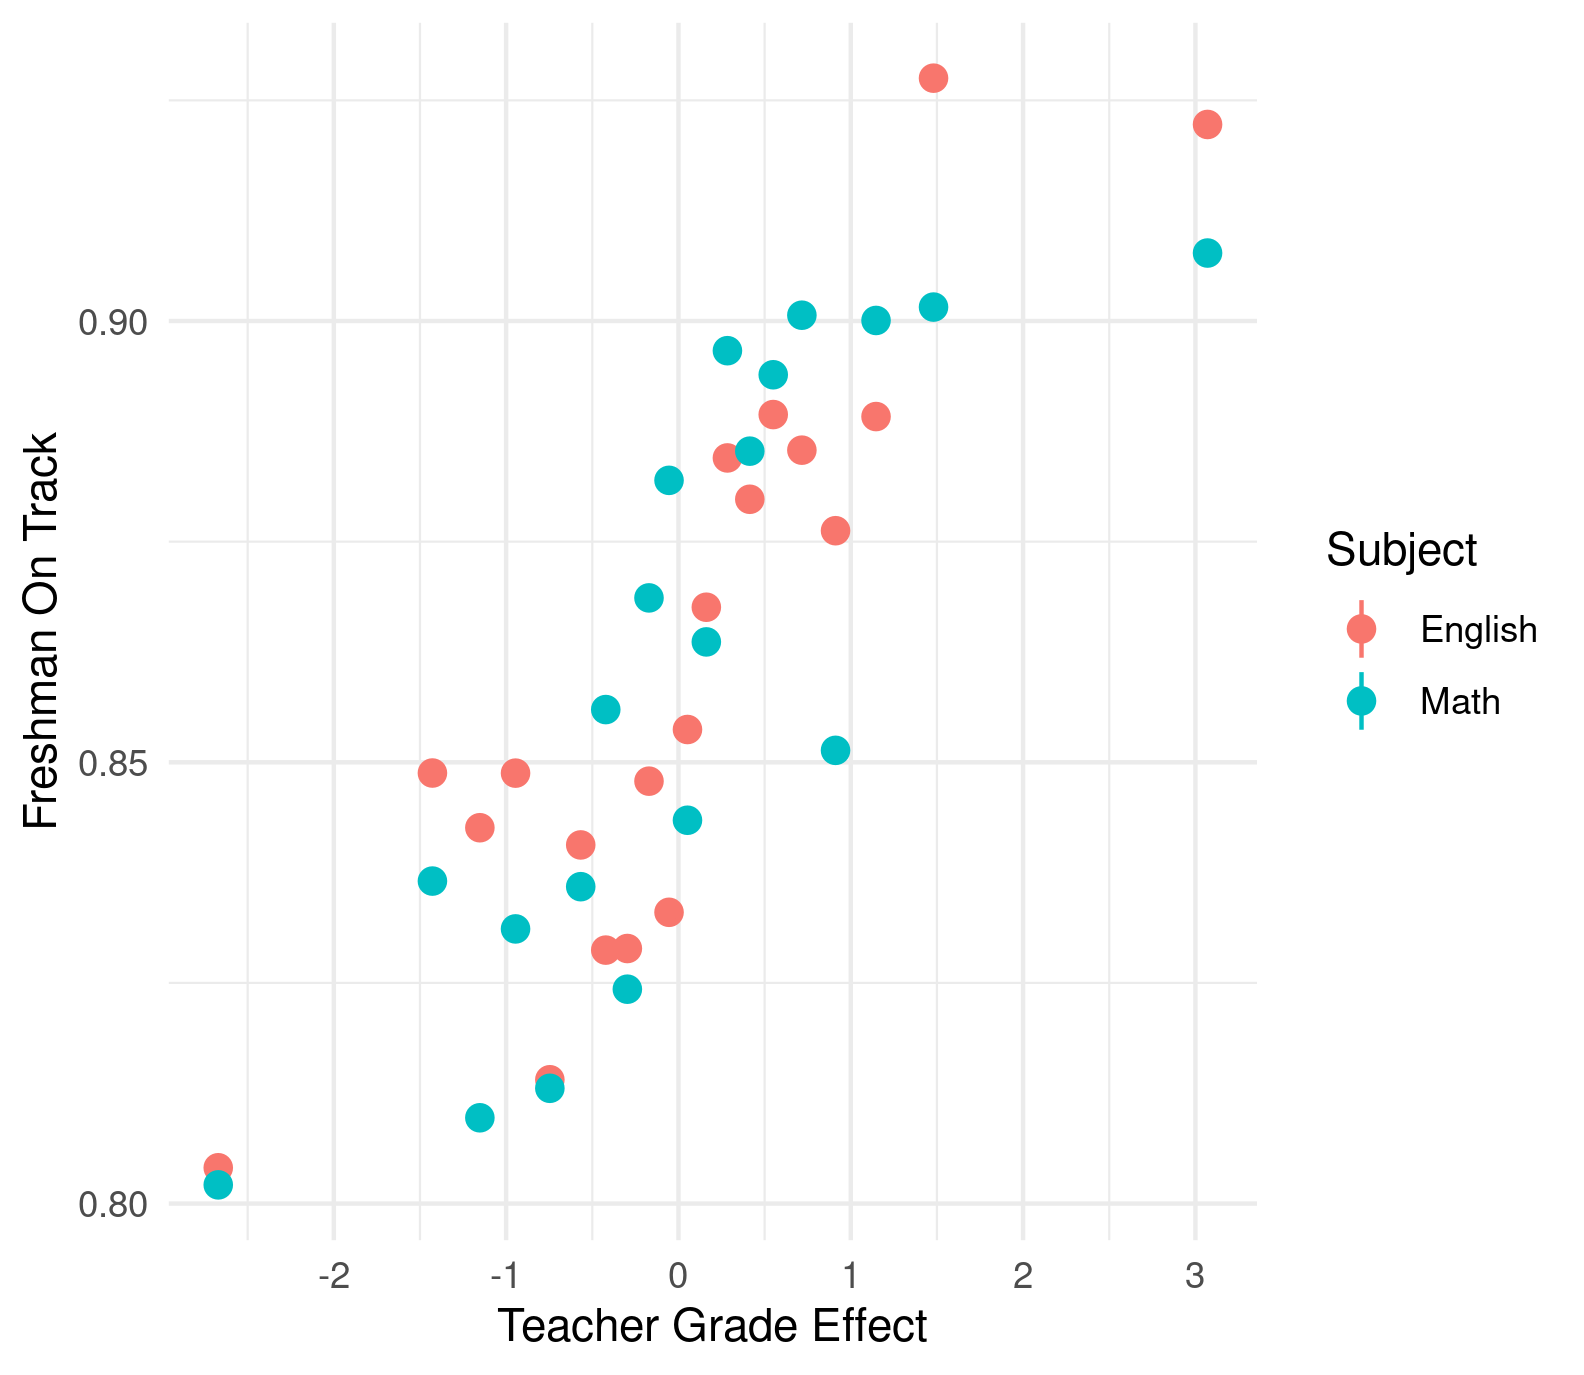
\includegraphics[width=\textwidth]{/Users/roymckenzie/Dropbox/Thesis/ECON/Output/dFreshOnTrack_scatter.png}
         \caption{Freshman on Track}
         \label{fig:dFreshOnTrack}
     \end{subfigure}
     \hfill
     \begin{subfigure}[b]{0.4\textwidth}
         \centering
         \includegraphics[width=\textwidth]{/Users/roymckenzie/Dropbox/Thesis/ECON/Output/freshCoreGpa_scatter.png}
         \caption{Freshman Core GPA}
         \label{fig:freshCoreGpa}
     \end{subfigure}\\

     \begin{subfigure}[b]{0.4\textwidth}
         \centering
         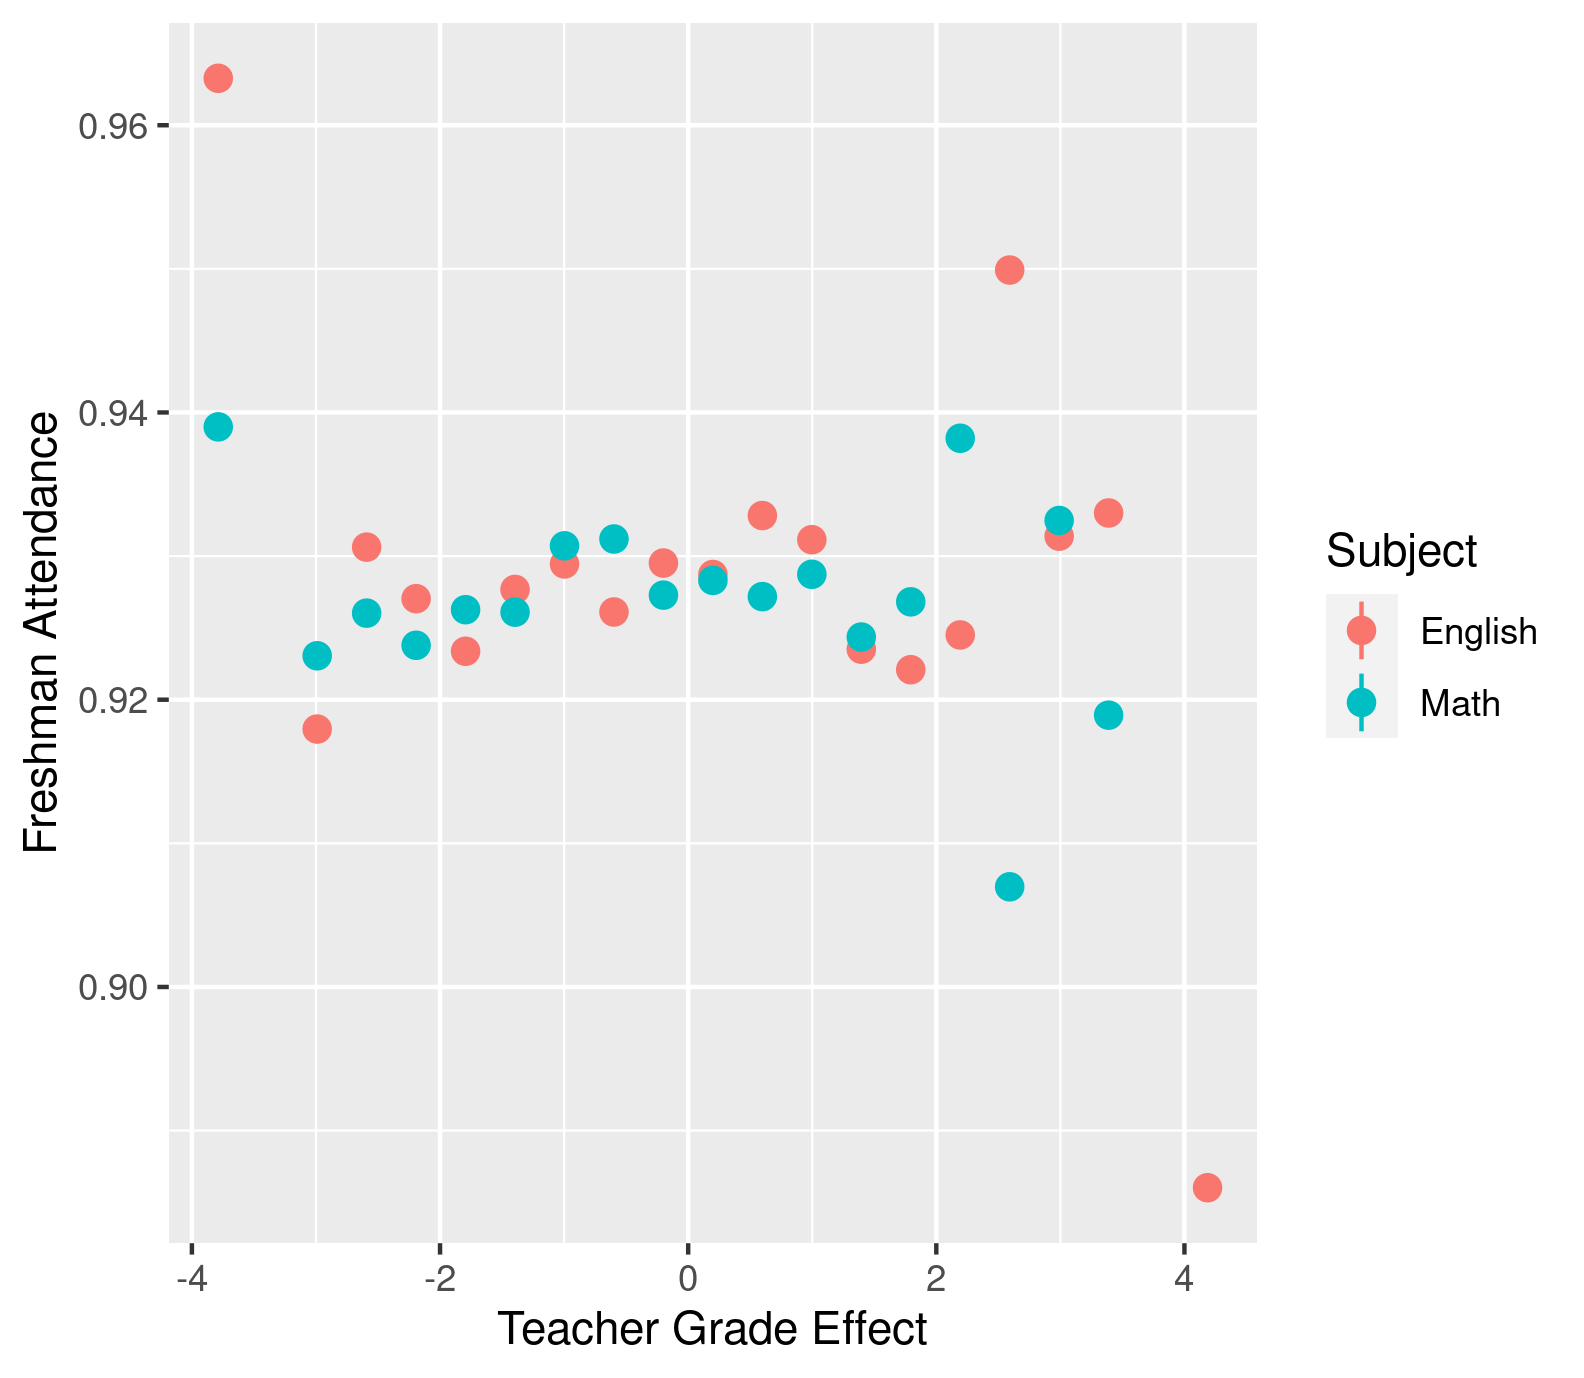
\includegraphics[width=\textwidth]{/Users/roymckenzie/Dropbox/Thesis/ECON/Output/pFreshAttendance_scatter.png}
         \caption{Freshman Attendance}
         \label{fig:pFreshAttendance}
     \end{subfigure}
        \caption{Freshman Year Outcomes}
        \label{fig:fresh}
\end{figure}

\subsection*{Course Taking Outcomes}

For the course outcomes, Table~\ref{tab:course_out} displays a significant effect only of English teacher grade effect on the number of AP courses taken after Freshman year. 


% Table created by stargazer v.5.2.2 by Marek Hlavac, Harvard University. E-mail: hlavac at fas.harvard.edu
% Date and time: Tue, May 11, 2021 - 01:28:34 PM
% Requires LaTeX packages: dcolumn 
\begin{table}[!htbp] \centering 
  \caption{Impact of Standardized Teacher Grade Effects on Course Taking Patterns} 
  \label{tab:course_out} 
\scriptsize 
\begin{tabular}{@{\extracolsep{5pt}}lD{.}{.}{-3} D{.}{.}{-3} D{.}{.}{-3} D{.}{.}{-3} } 
\\[-1.8ex]\hline 
\hline \\[-1.8ex] 
\\[-1.8ex] & \multicolumn{2}{c}{N. AP Courses After Freshman Year} & \multicolumn{2}{c}{N. Honors Courses After Freshman Year} \\ 
 & \multicolumn{1}{c}{Math} & \multicolumn{1}{c}{English} & \multicolumn{1}{c}{Math} & \multicolumn{1}{c}{English} \\ 
\hline \\[-1.8ex] 
 Teacher Grade Effect & 0.023 & -0.300^{*} & 0.801 & 0.108 \\ 
  & (0.155) & (0.155) & (0.632) & (0.622) \\ 
  & & & & \\ 
Year Dummies & \multicolumn{1}{c}{Yes} & \multicolumn{1}{c}{Yes} & \multicolumn{1}{c}{Yes} & \multicolumn{1}{c}{Yes} \\ 
Mean (All Years) & 3.493 & 3.354 & 12.831 & 12.86 \\ 
Observations & \multicolumn{1}{c}{883} & \multicolumn{1}{c}{869} & \multicolumn{1}{c}{883} & \multicolumn{1}{c}{869} \\ 
\hline \\[-1.8ex] 
\textit{Notes:} & \multicolumn{4}{r}{$^{***}$Significant at the 1 percent level.} \\ 
 & \multicolumn{4}{r}{$^{**}$Significant at the 5 percent level.} \\ 
 & \multicolumn{4}{r}{$^{*}$Significant at the 10 percent level.} \\ 
 & \multicolumn{4}{r}{This table displays the outcome of regressing residualized} \\ 
 & \multicolumn{4}{r}{outcomes on teacher grade effects by subject and outcome,} \\ 
 & \multicolumn{4}{r}{allowing for year fixed effects. Heteroskedasticity robust} \\ 
 & \multicolumn{4}{r}{standard errors are used} \\ 
\end{tabular} 
\end{table} 


\begin{figure}
     \centering
     \begin{subfigure}[b]{0.45\textwidth}
         \centering
         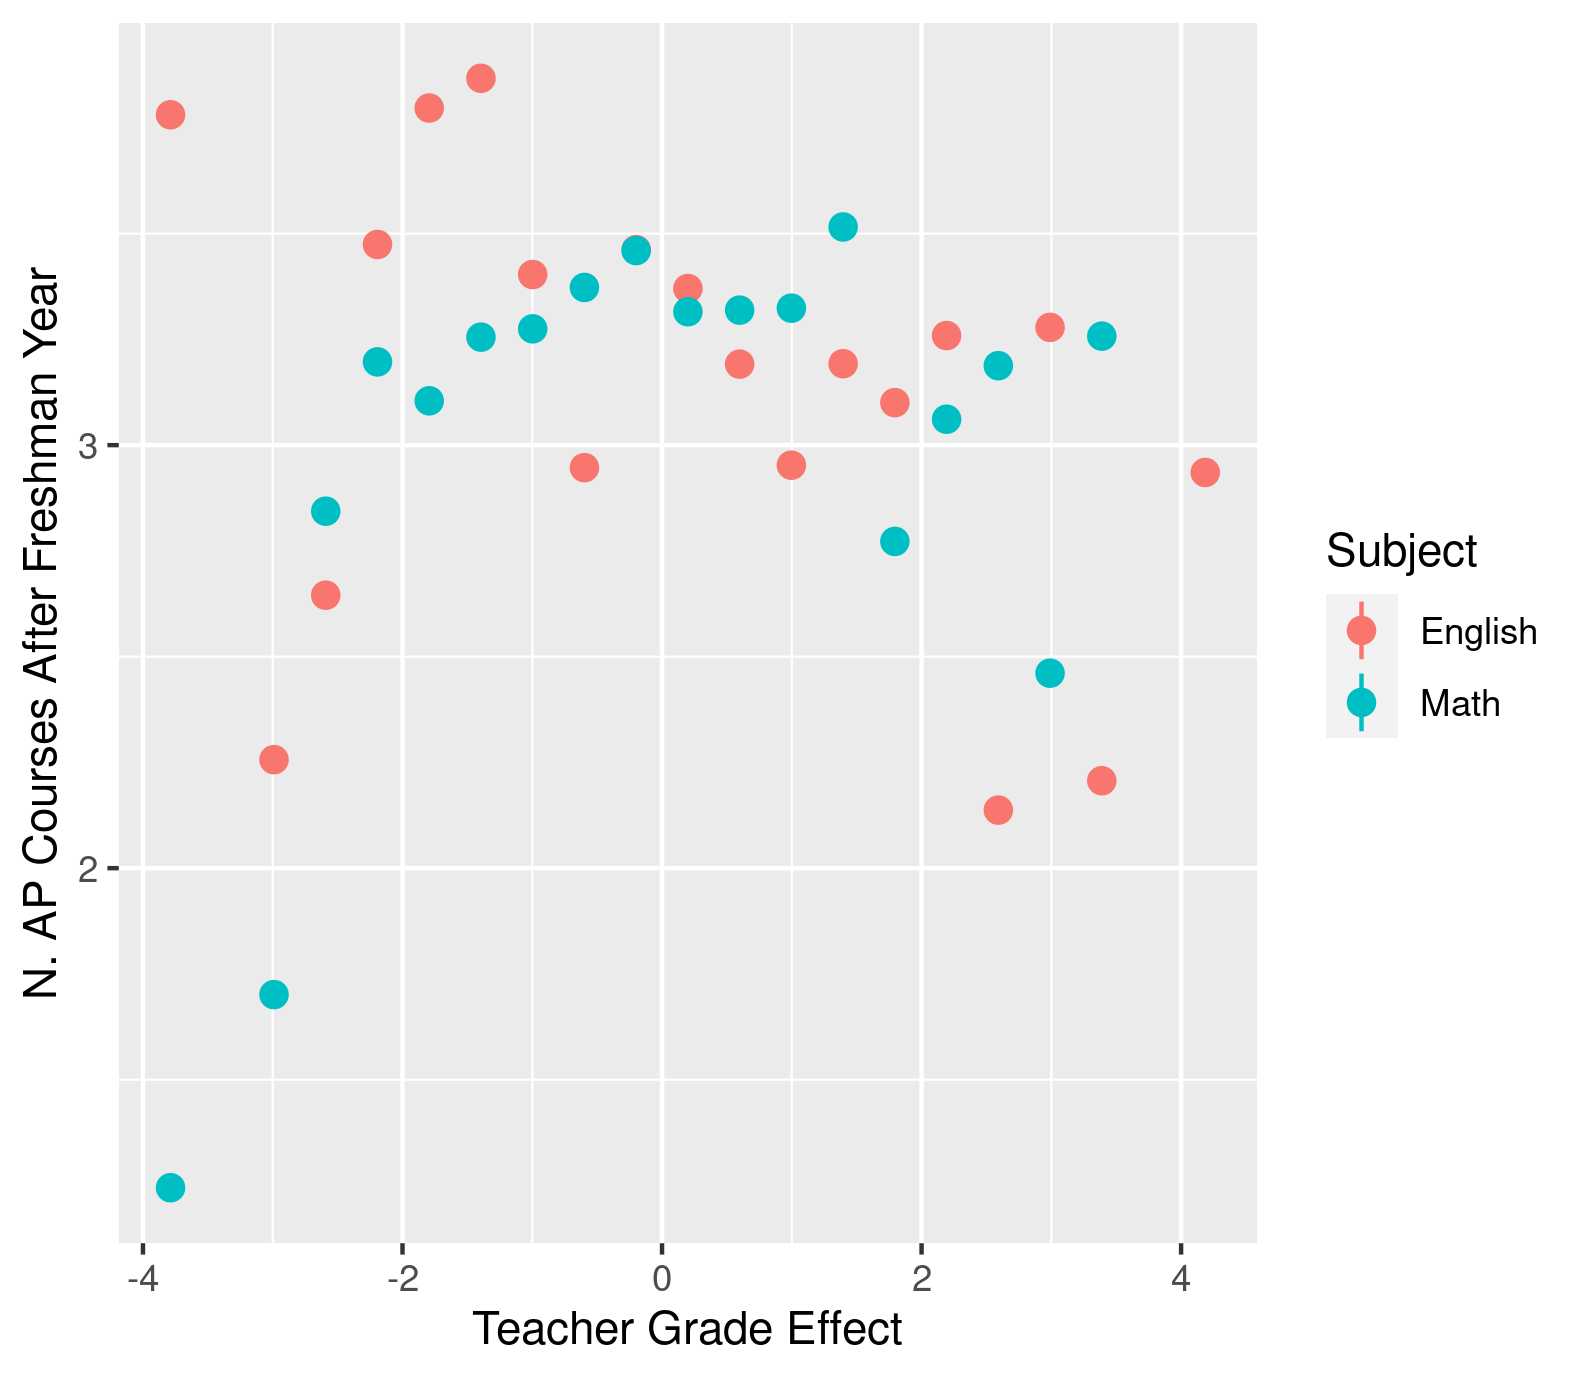
\includegraphics[width=\textwidth]{/Users/roymckenzie/Dropbox/Thesis/ECON/Output/nAPCourses4yr_scatter.png}
         \caption{N. AP Courses after Freshman Year}
         \label{fig:nAPCourses4yr}
     \end{subfigure}
     \hfill
     \begin{subfigure}[b]{0.45\textwidth}
         \centering
         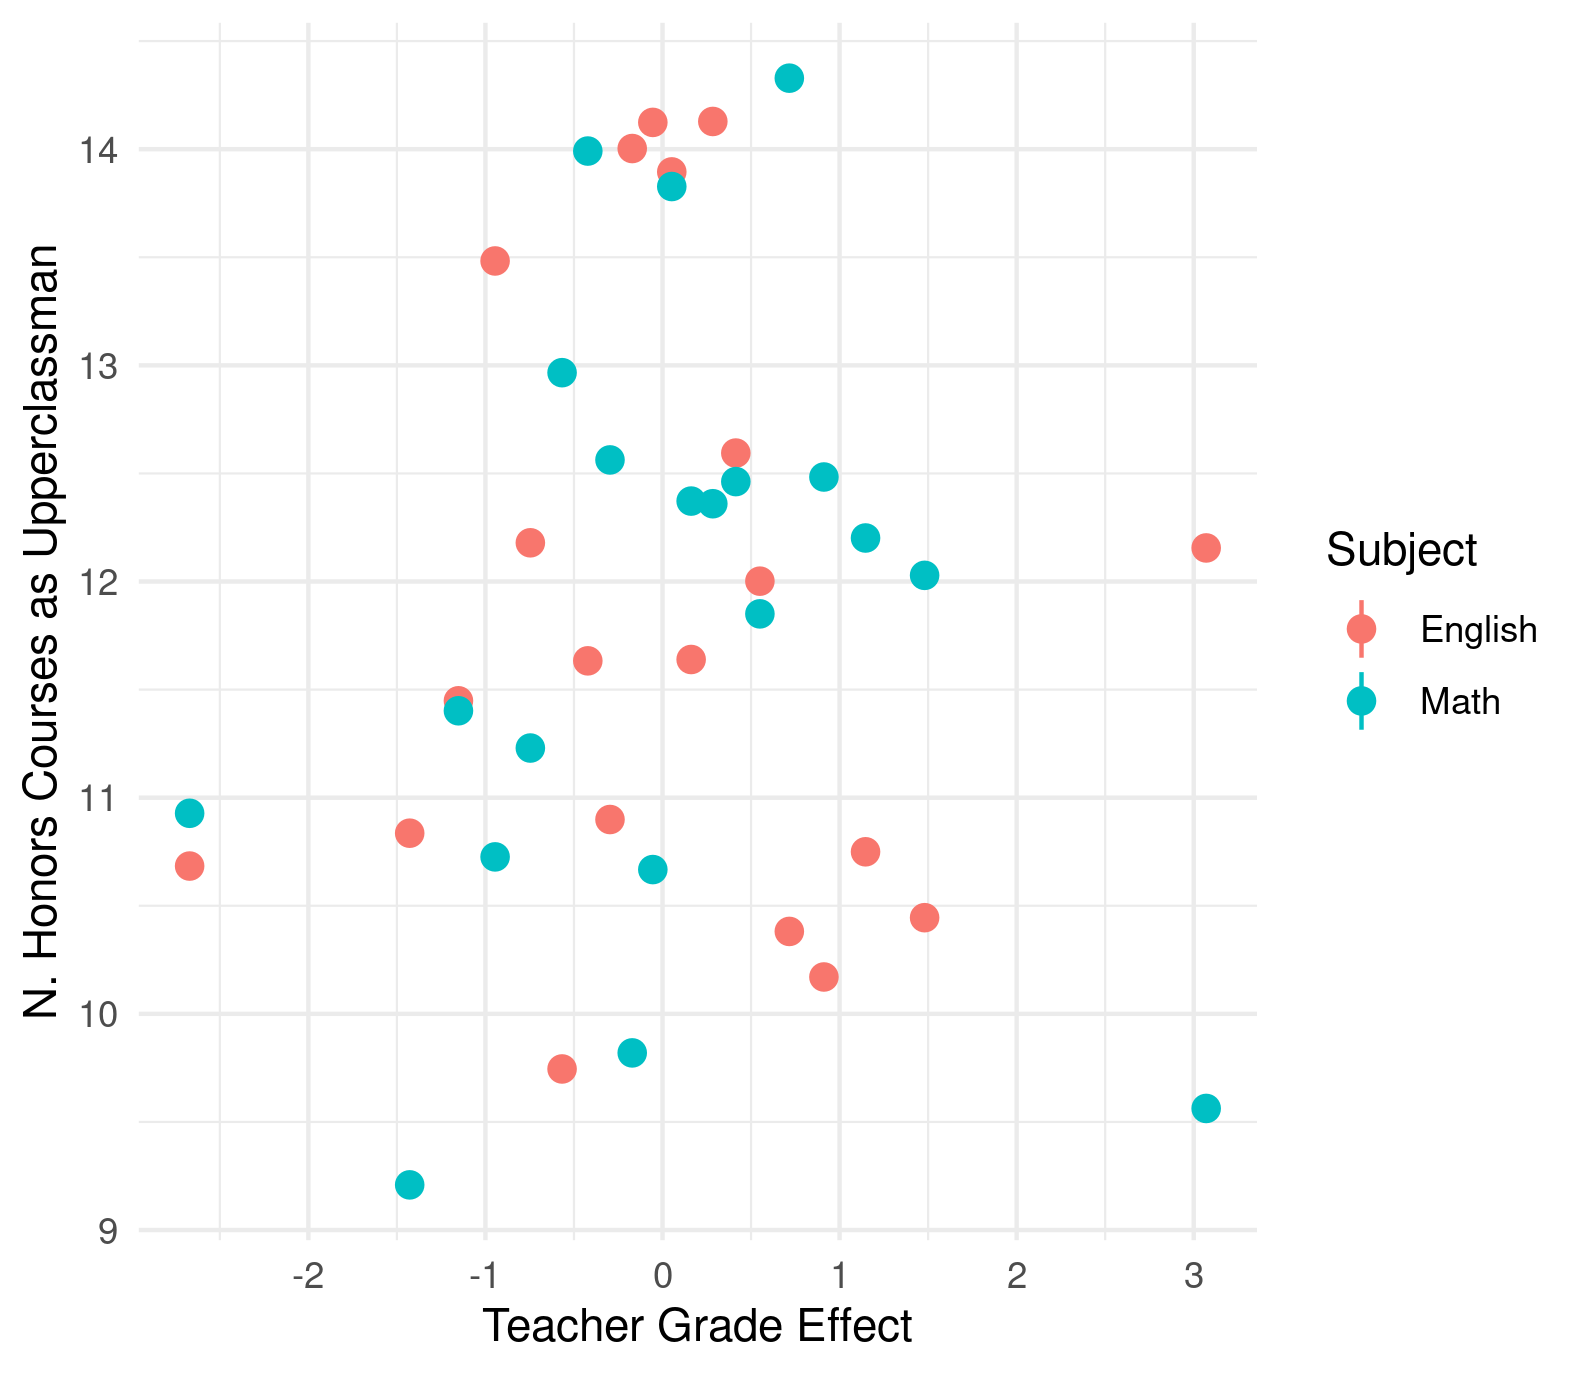
\includegraphics[width=\textwidth]{/Users/roymckenzie/Dropbox/Thesis/ECON/Output/n_honors_after_fresh_scatter.png}
         \caption{N. Honors Courses after Freshman Year}
         \label{fig:freshCoreGpa}
     \end{subfigure}
      \caption{Course Taking Outcomes}
      \label{fig:course}
\end{figure}

\subsection*{Later Academic Outcomes}

Again, in Table~\ref{tab:academic_out}, we see a likely-endogenous effect of teacher grade effect on both core and overall graduating GPA. 


% Table created by stargazer v.5.2.2 by Marek Hlavac, Harvard University. E-mail: hlavac at fas.harvard.edu
% Date and time: Fri, May 14, 2021 - 09:46:06 PM
% Requires LaTeX packages: dcolumn 
\begin{table}[!htbp] \centering 
  \caption{Impact of Standardized Teacher Grade Effects on Academic Outcomes} 
  \label{tab:academic_out} 
\scriptsize 
\begin{tabular}{@{\extracolsep{5pt}}lD{.}{.}{-3} D{.}{.}{-3} D{.}{.}{-3} D{.}{.}{-3} D{.}{.}{-3} D{.}{.}{-3} } 
\\[-1.8ex]\hline 
\hline \\[-1.8ex] 
\\[-1.8ex] & \multicolumn{2}{c}{ACT/SAT Score (ACT Scale)} & \multicolumn{2}{c}{Graduating Core GPA} & \multicolumn{2}{c}{Graduating Overall GPA} \\ 
 & \multicolumn{1}{c}{Math} & \multicolumn{1}{c}{English} & \multicolumn{1}{c}{Math} & \multicolumn{1}{c}{English} & \multicolumn{1}{c}{Math} & \multicolumn{1}{c}{English} \\ 
\hline \\[-1.8ex] 
 Teacher Grade Effect & -0.002 & -0.018 & 0.019^{***} & 0.023^{***} & 0.020^{***} & 0.017^{***} \\ 
  & (0.014) & (0.013) & (0.004) & (0.004) & (0.004) & (0.004) \\ 
  & & & & & & \\ 
Year Dummies & \multicolumn{1}{c}{Yes} & \multicolumn{1}{c}{Yes} & \multicolumn{1}{c}{Yes} & \multicolumn{1}{c}{Yes} & \multicolumn{1}{c}{Yes} & \multicolumn{1}{c}{Yes} \\ 
Mean (All Years) & 19.476 & 19.422 & 2.424 & 2.421 & 2.572 & 2.569 \\ 
Observations & \multicolumn{1}{c}{28,049} & \multicolumn{1}{c}{29,472} & \multicolumn{1}{c}{31,214} & \multicolumn{1}{c}{32,740} & \multicolumn{1}{c}{31,214} & \multicolumn{1}{c}{32,740} \\ 
\hline \\[-1.8ex] 
\textit{Notes:} & \multicolumn{6}{r}{$^{***}$Significant at the 1 percent level.} \\ 
 & \multicolumn{6}{r}{$^{**}$Significant at the 5 percent level.} \\ 
 & \multicolumn{6}{r}{$^{*}$Significant at the 10 percent level.} \\ 
 & \multicolumn{6}{r}{This table displays the outcome of regressing residualized} \\ 
 & \multicolumn{6}{r}{outcomes on teacher grade effects by subject and outcome,} \\ 
 & \multicolumn{6}{r}{allowing for year fixed effects. Heteroskedasticity robust} \\ 
 & \multicolumn{6}{r}{standard errors are used} \\ 
\end{tabular} 
\end{table} 


\begin{figure}
     \centering
     \begin{subfigure}[b]{0.4\textwidth}
         \centering
         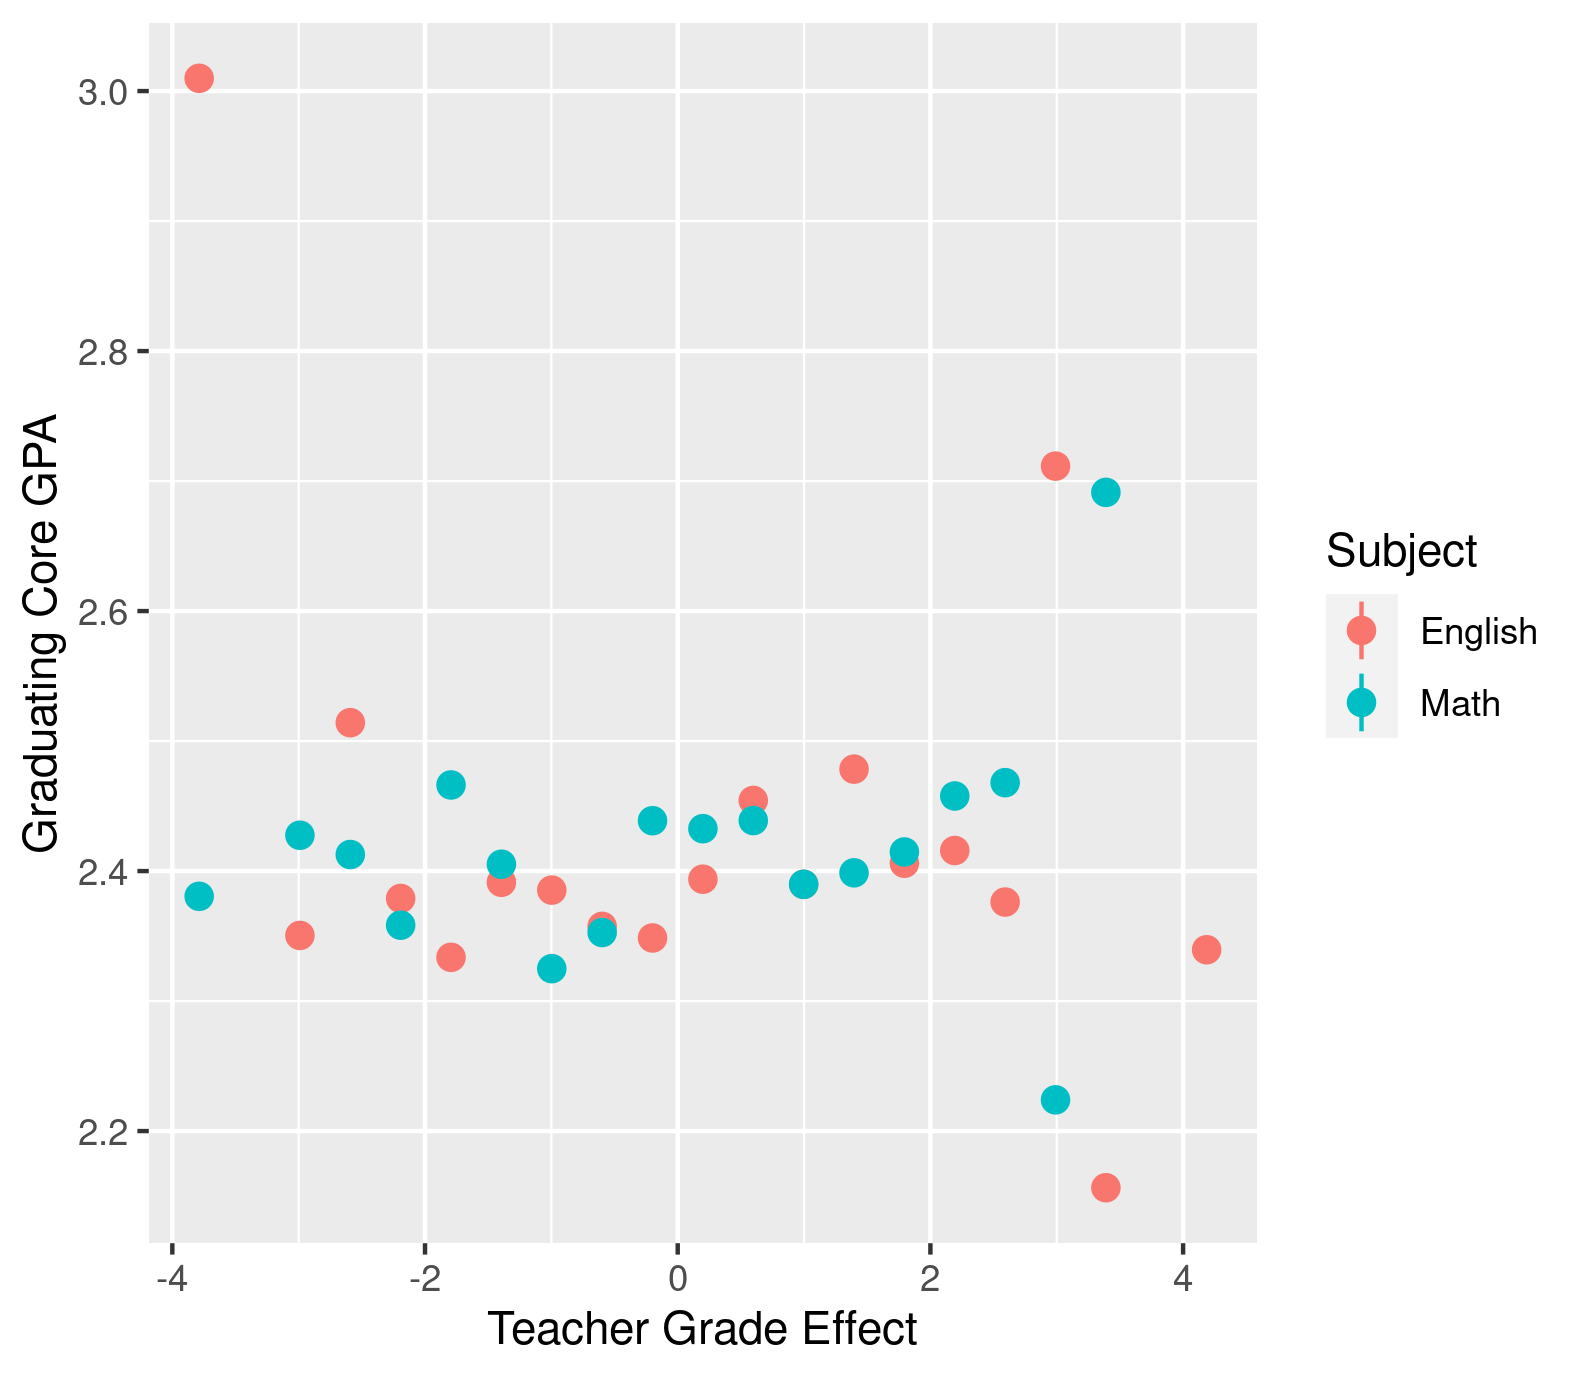
\includegraphics[width=\textwidth]{/Users/roymckenzie/Dropbox/Thesis/ECON/Output/gradCumCoreGPA_scatter.png}
         \caption{College Entrance Exam (ACT Units)}
         \label{fig:highACT_EQUIV}
     \end{subfigure}
     \hfill
     \begin{subfigure}[b]{0.4\textwidth}
         \centering
         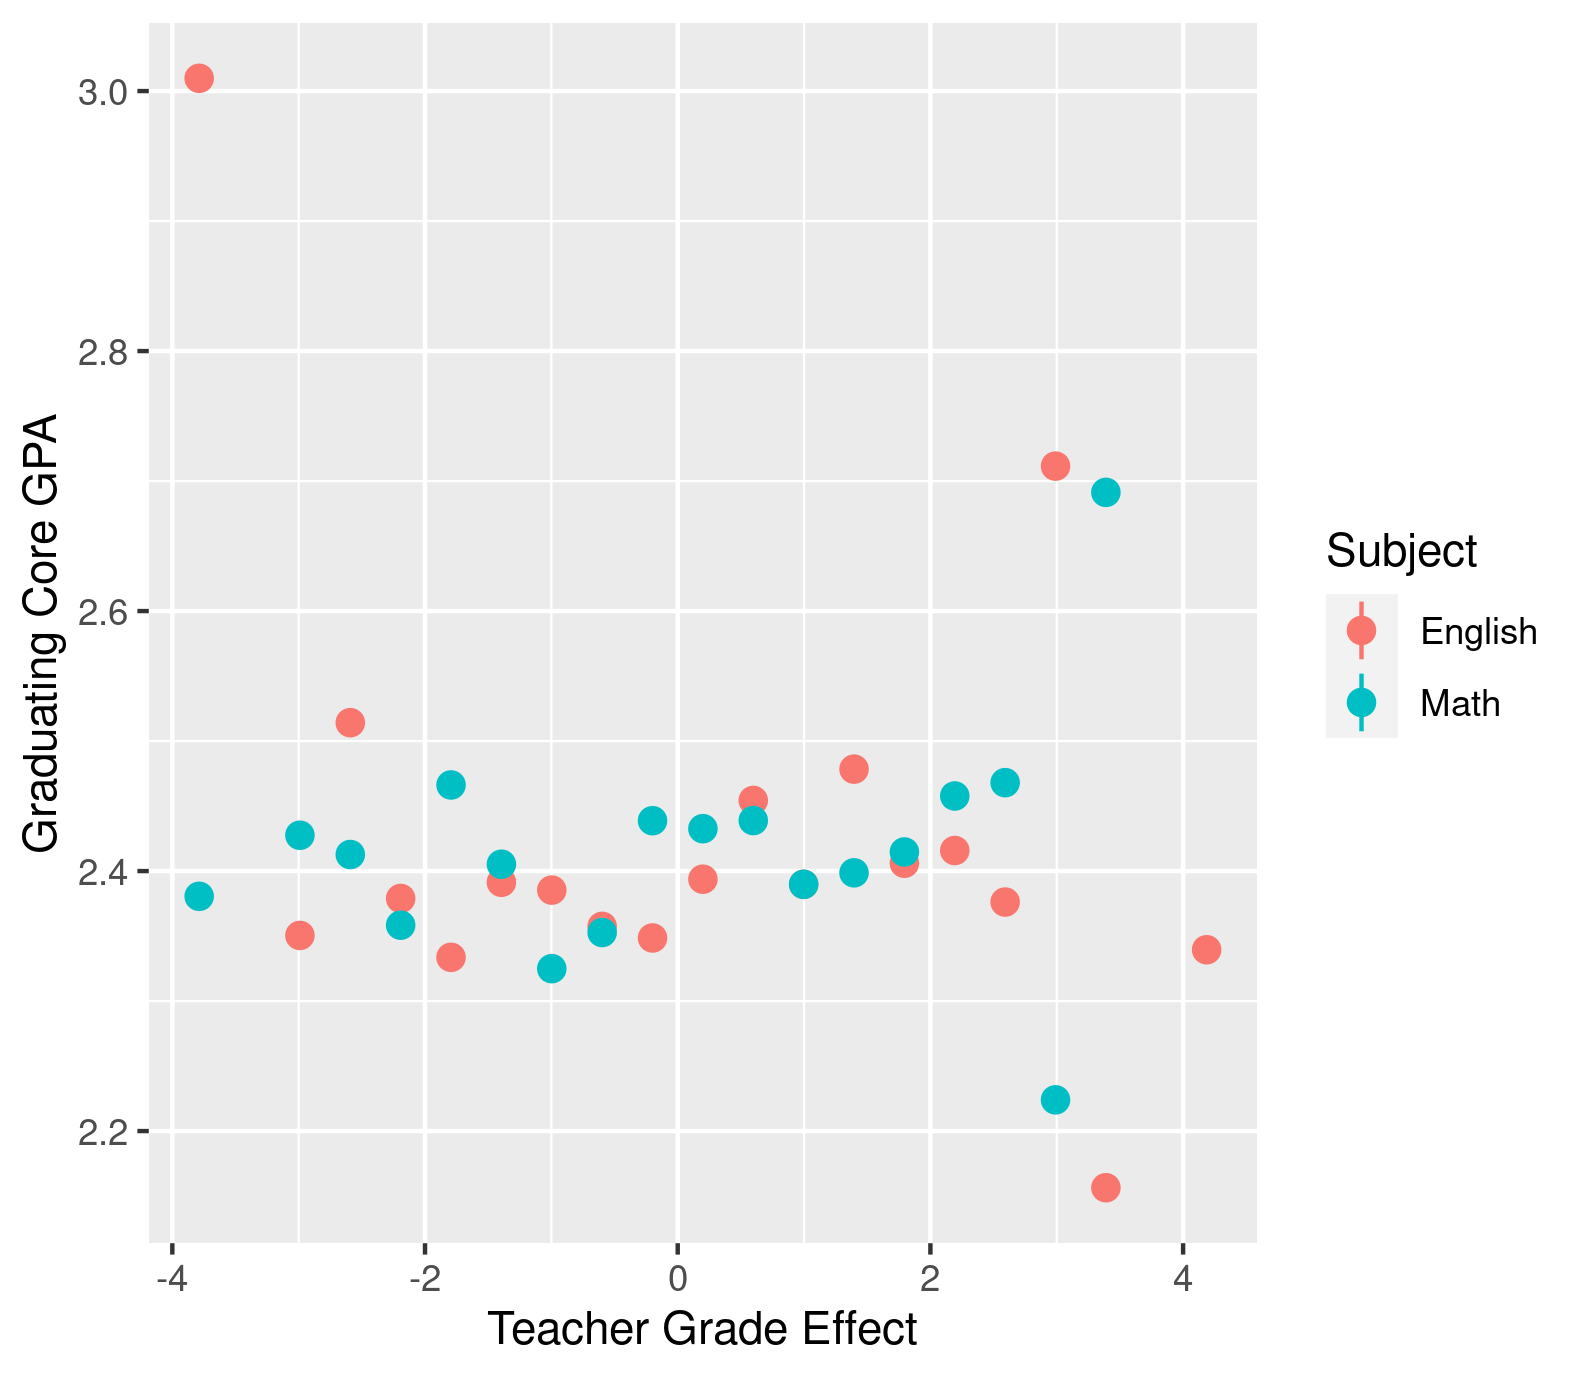
\includegraphics[width=\textwidth]{/Users/roymckenzie/Dropbox/Thesis/ECON/Output/gradCumCoreGPA_scatter.png}
         \caption{Graduating Core GPA}
         \label{fig:gradCumCoreGPA}
     \end{subfigure}\\

     \begin{subfigure}[b]{0.4\textwidth}
         \centering
         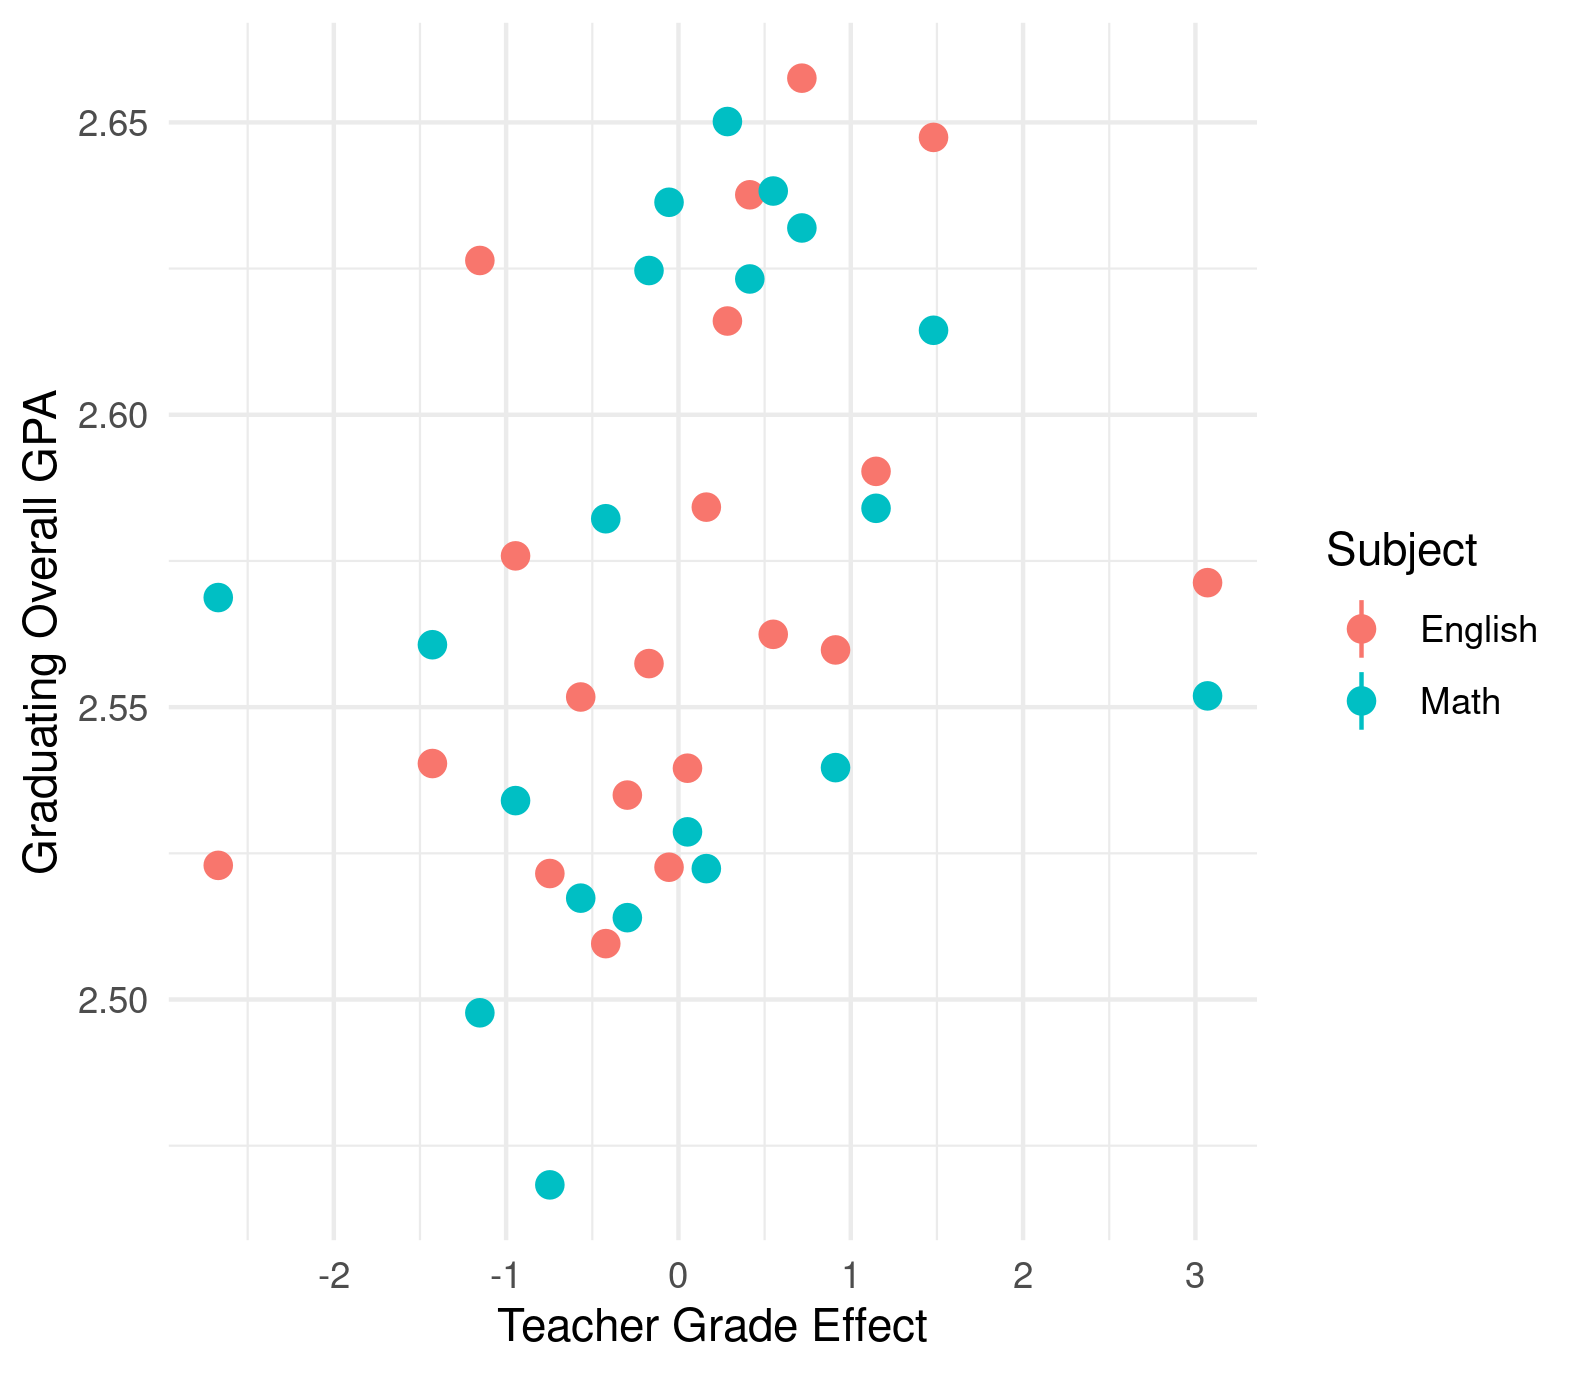
\includegraphics[width=\textwidth]{/Users/roymckenzie/Dropbox/Thesis/ECON/Output/gradCumOverallGPA_scatter.png}
         \caption{Graduating Overall GPA}
         \label{fig:gradCumOverallGPA}
     \end{subfigure}
    \caption{Long-Term Academic Outcomes}
    \label{fig:academic}
\end{figure}

\subsection*{Post-Secondary Outcomes}

In Table~\ref{tab:long_out} we see a significant impact of Freshman year math teacher grade efect on immediate college enrollment. The magnitude of this effect, however, is so small as to be negligible. 


% Table created by stargazer v.5.2.2 by Marek Hlavac, Harvard University. E-mail: hlavac at fas.harvard.edu
% Date and time: Fri, May 14, 2021 - 09:47:04 PM
% Requires LaTeX packages: dcolumn 
\begin{table}[!htbp] \centering 
  \caption{Impact of Standardized Teacher Grade Effects on Long Term Outcomes} 
  \label{tab:long_out} 
\scriptsize 
\begin{tabular}{@{\extracolsep{5pt}}lD{.}{.}{-3} D{.}{.}{-3} D{.}{.}{-3} D{.}{.}{-3} D{.}{.}{-3} D{.}{.}{-3} } 
\\[-1.8ex]\hline 
\hline \\[-1.8ex] 
\\[-1.8ex] & \multicolumn{2}{c}{Graduate HS in 4 Years} & \multicolumn{2}{c}{Immediately Enrolled in College} & \multicolumn{2}{c}{On Time College Graduation} \\ 
 & \multicolumn{1}{c}{Math} & \multicolumn{1}{c}{English} & \multicolumn{1}{c}{Math} & \multicolumn{1}{c}{English} & \multicolumn{1}{c}{Math} & \multicolumn{1}{c}{English} \\ 
\hline \\[-1.8ex] 
 Teacher Grade Effect & -0.001 & -0.000 & -0.005^{*} & -0.002 & 0.001 & -0.001 \\ 
  & (0.002) & (0.002) & (0.003) & (0.003) & (0.002) & (0.002) \\ 
  & & & & & & \\ 
Year Dummies & \multicolumn{1}{c}{Yes} & \multicolumn{1}{c}{Yes} & \multicolumn{1}{c}{Yes} & \multicolumn{1}{c}{Yes} & \multicolumn{1}{c}{Yes} & \multicolumn{1}{c}{Yes} \\ 
Mean (All Years) & 0.89 & 0.889 & 0.663 & 0.66 & 0.178 & 0.176 \\ 
Observations & \multicolumn{1}{c}{29,180} & \multicolumn{1}{c}{30,658} & \multicolumn{1}{c}{27,170} & \multicolumn{1}{c}{28,538} & \multicolumn{1}{c}{27,170} & \multicolumn{1}{c}{28,538} \\ 
\hline \\[-1.8ex] 
\textit{Notes:} & \multicolumn{6}{r}{$^{***}$Significant at the 1 percent level.} \\ 
 & \multicolumn{6}{r}{$^{**}$Significant at the 5 percent level.} \\ 
 & \multicolumn{6}{r}{$^{*}$Significant at the 10 percent level.} \\ 
 & \multicolumn{6}{r}{This table displays the outcome of regressing residualized} \\ 
 & \multicolumn{6}{r}{outcomes on teacher grade effects by subject and outcome,} \\ 
 & \multicolumn{6}{r}{allowing for year fixed effects. Heteroskedasticity robust} \\ 
 & \multicolumn{6}{r}{standard errors are used} \\ 
\end{tabular} 
\end{table} 


\begin{figure}
     \centering
     \begin{subfigure}[b]{0.4\textwidth}
         \centering
         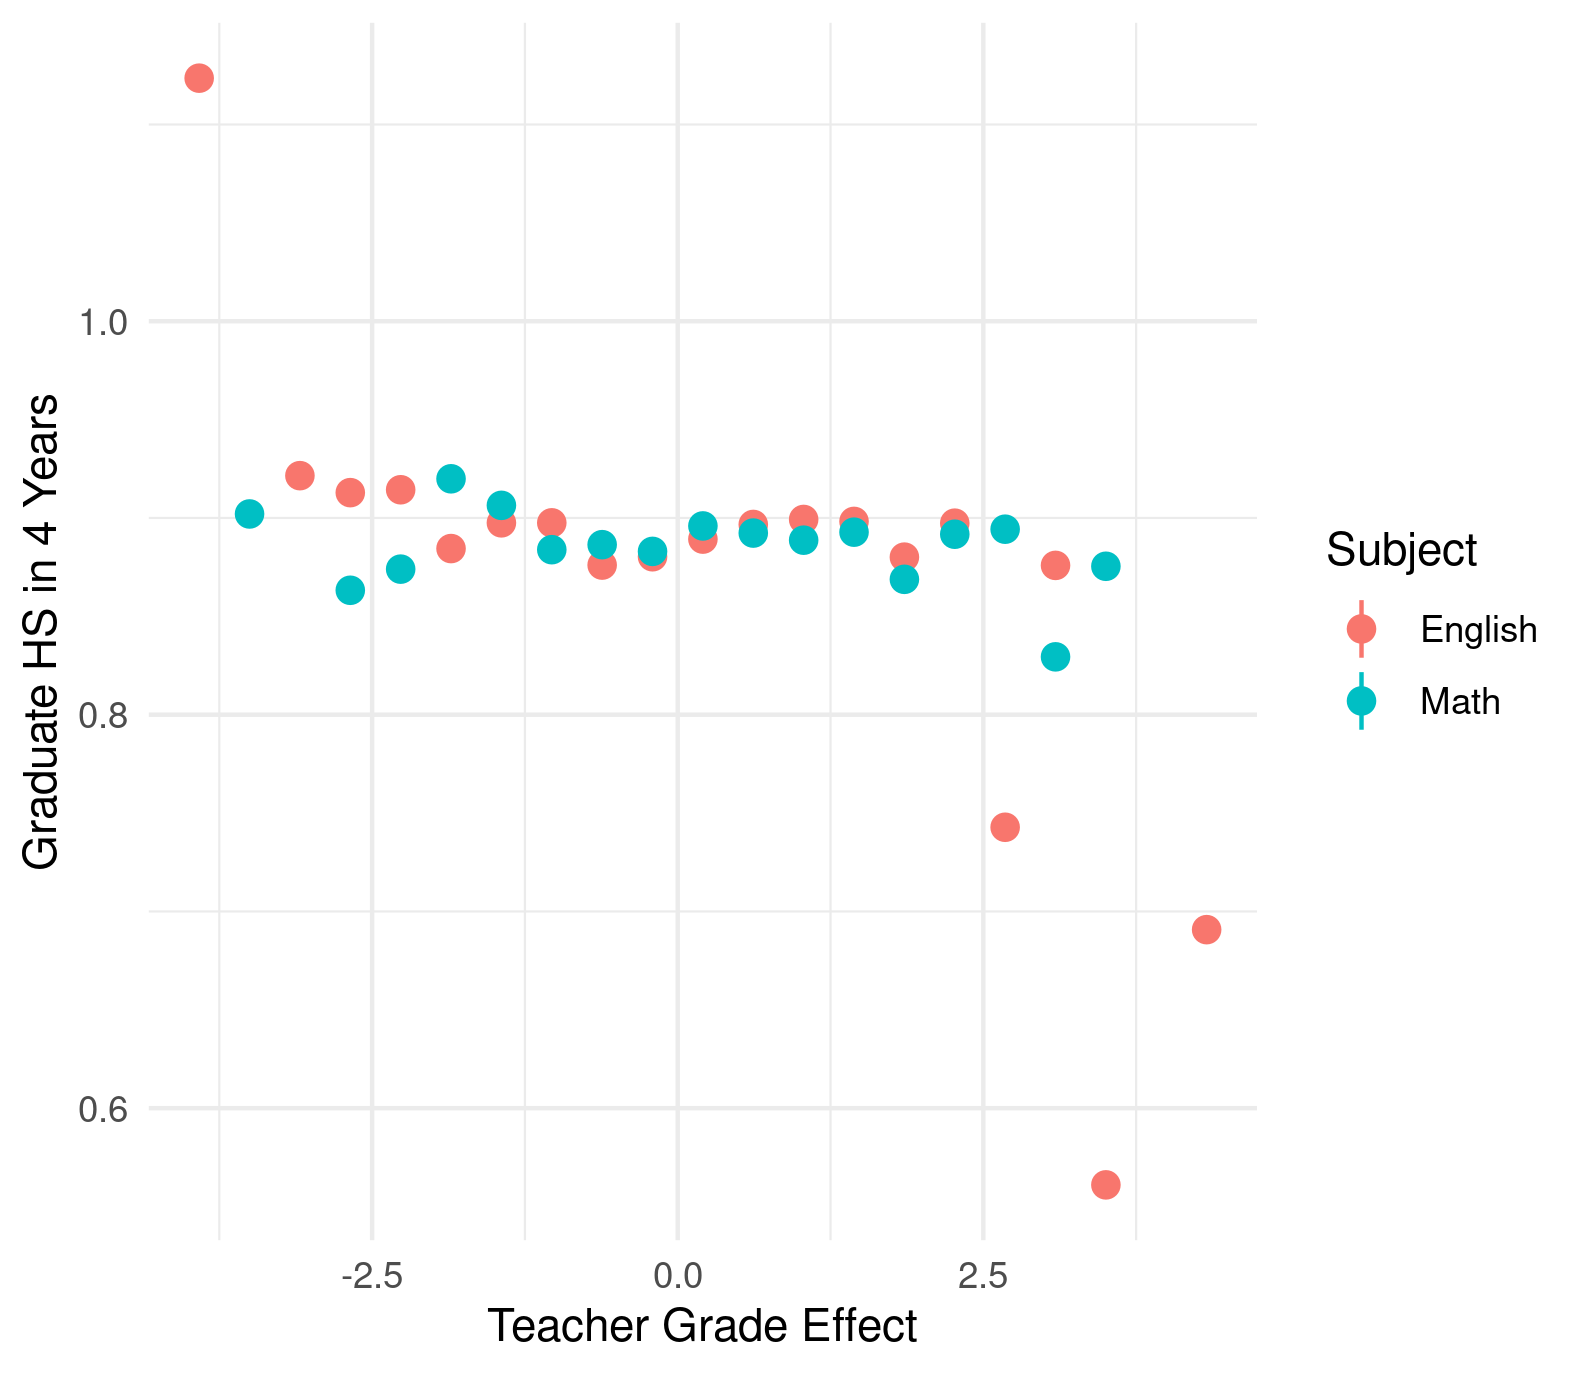
\includegraphics[width=\textwidth]{/Users/roymckenzie/Dropbox/Thesis/ECON/Output/dEarnAnyDip4yr_scatter.png}
         \caption{Graduating HS in 4 Years}
         \label{fig:dEarnAnyDip4yr}
     \end{subfigure}
     \hfill
     \begin{subfigure}[b]{0.4\textwidth}
         \centering
         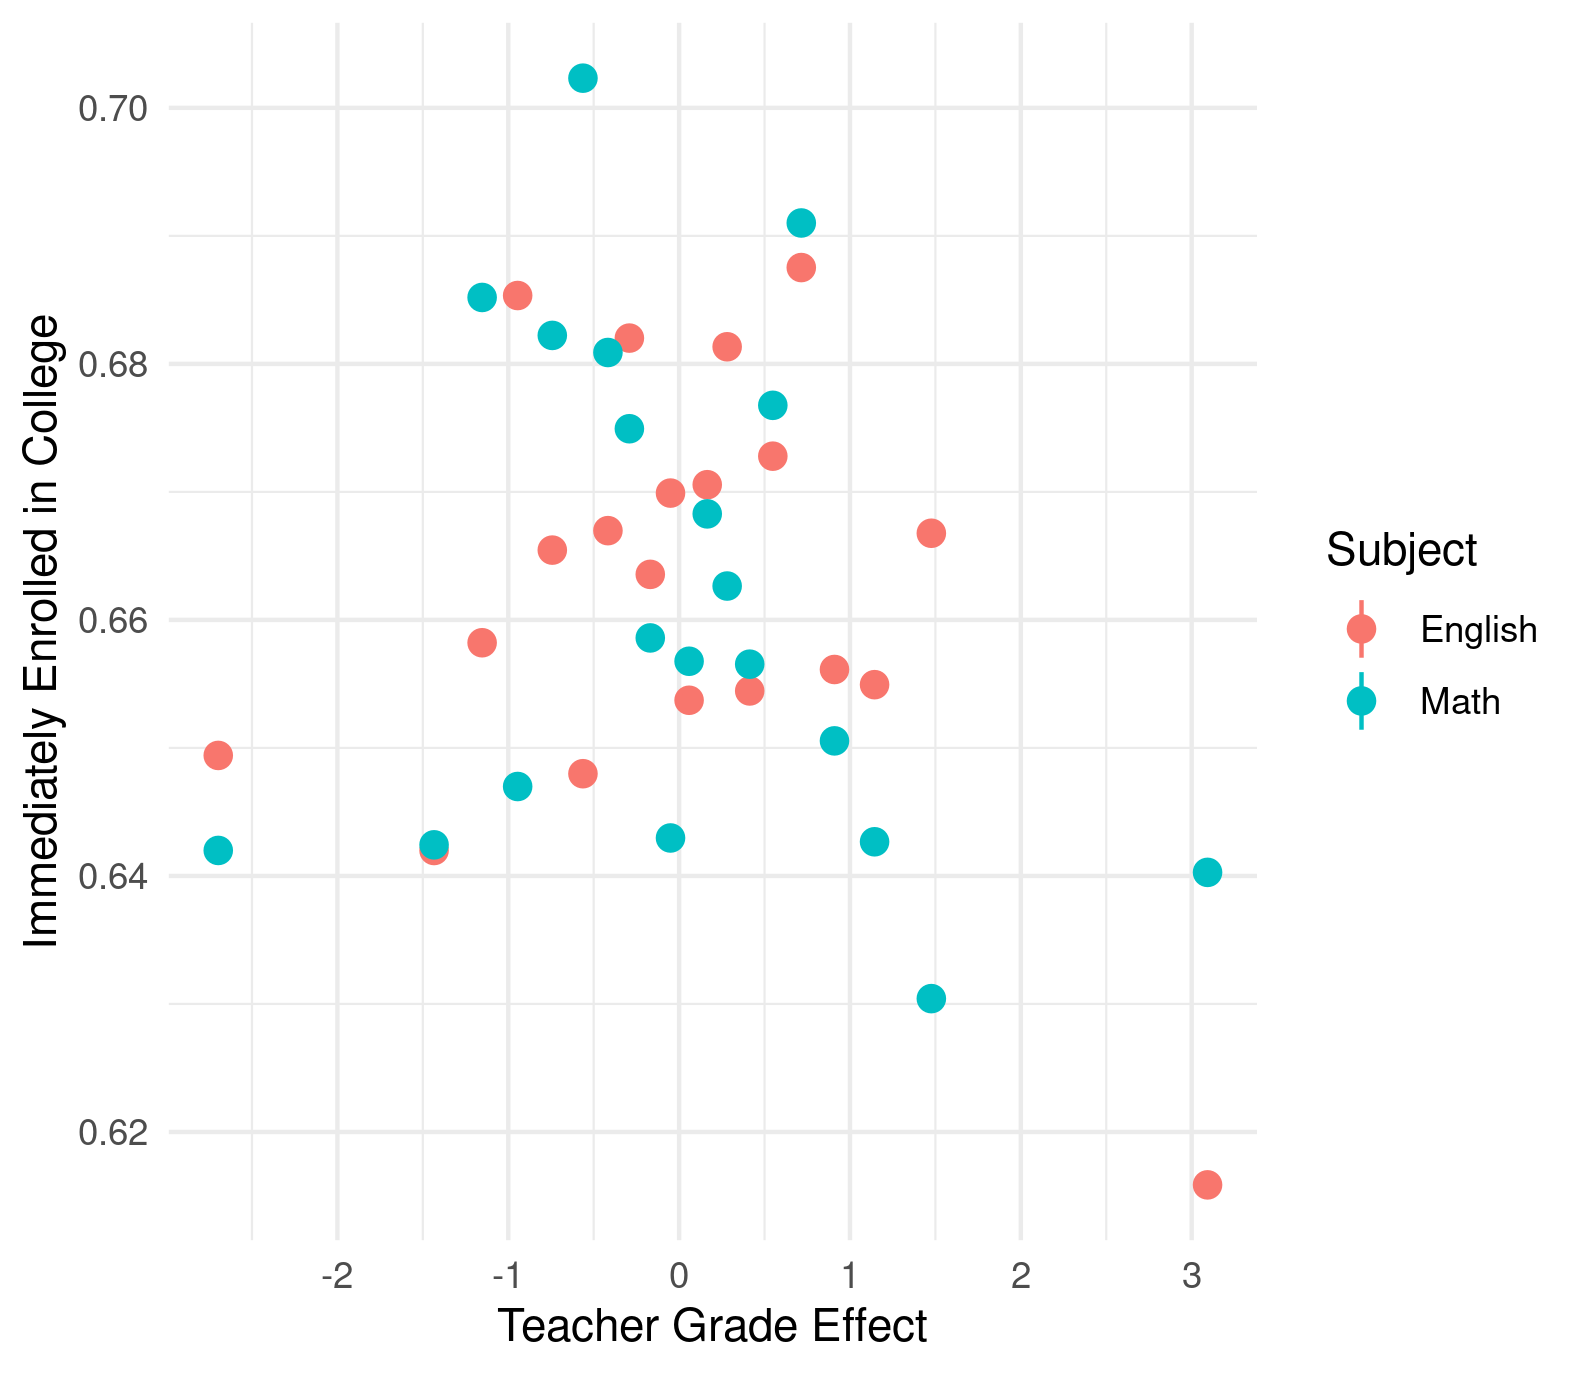
\includegraphics[width=\textwidth]{/Users/roymckenzie/Dropbox/Thesis/ECON/Output/immEnr_scatter.png}
         \caption{Immediate College Enrollment}
         \label{fig:immEnr}
     \end{subfigure}\\

     \begin{subfigure}[b]{0.4\textwidth}
         \centering
         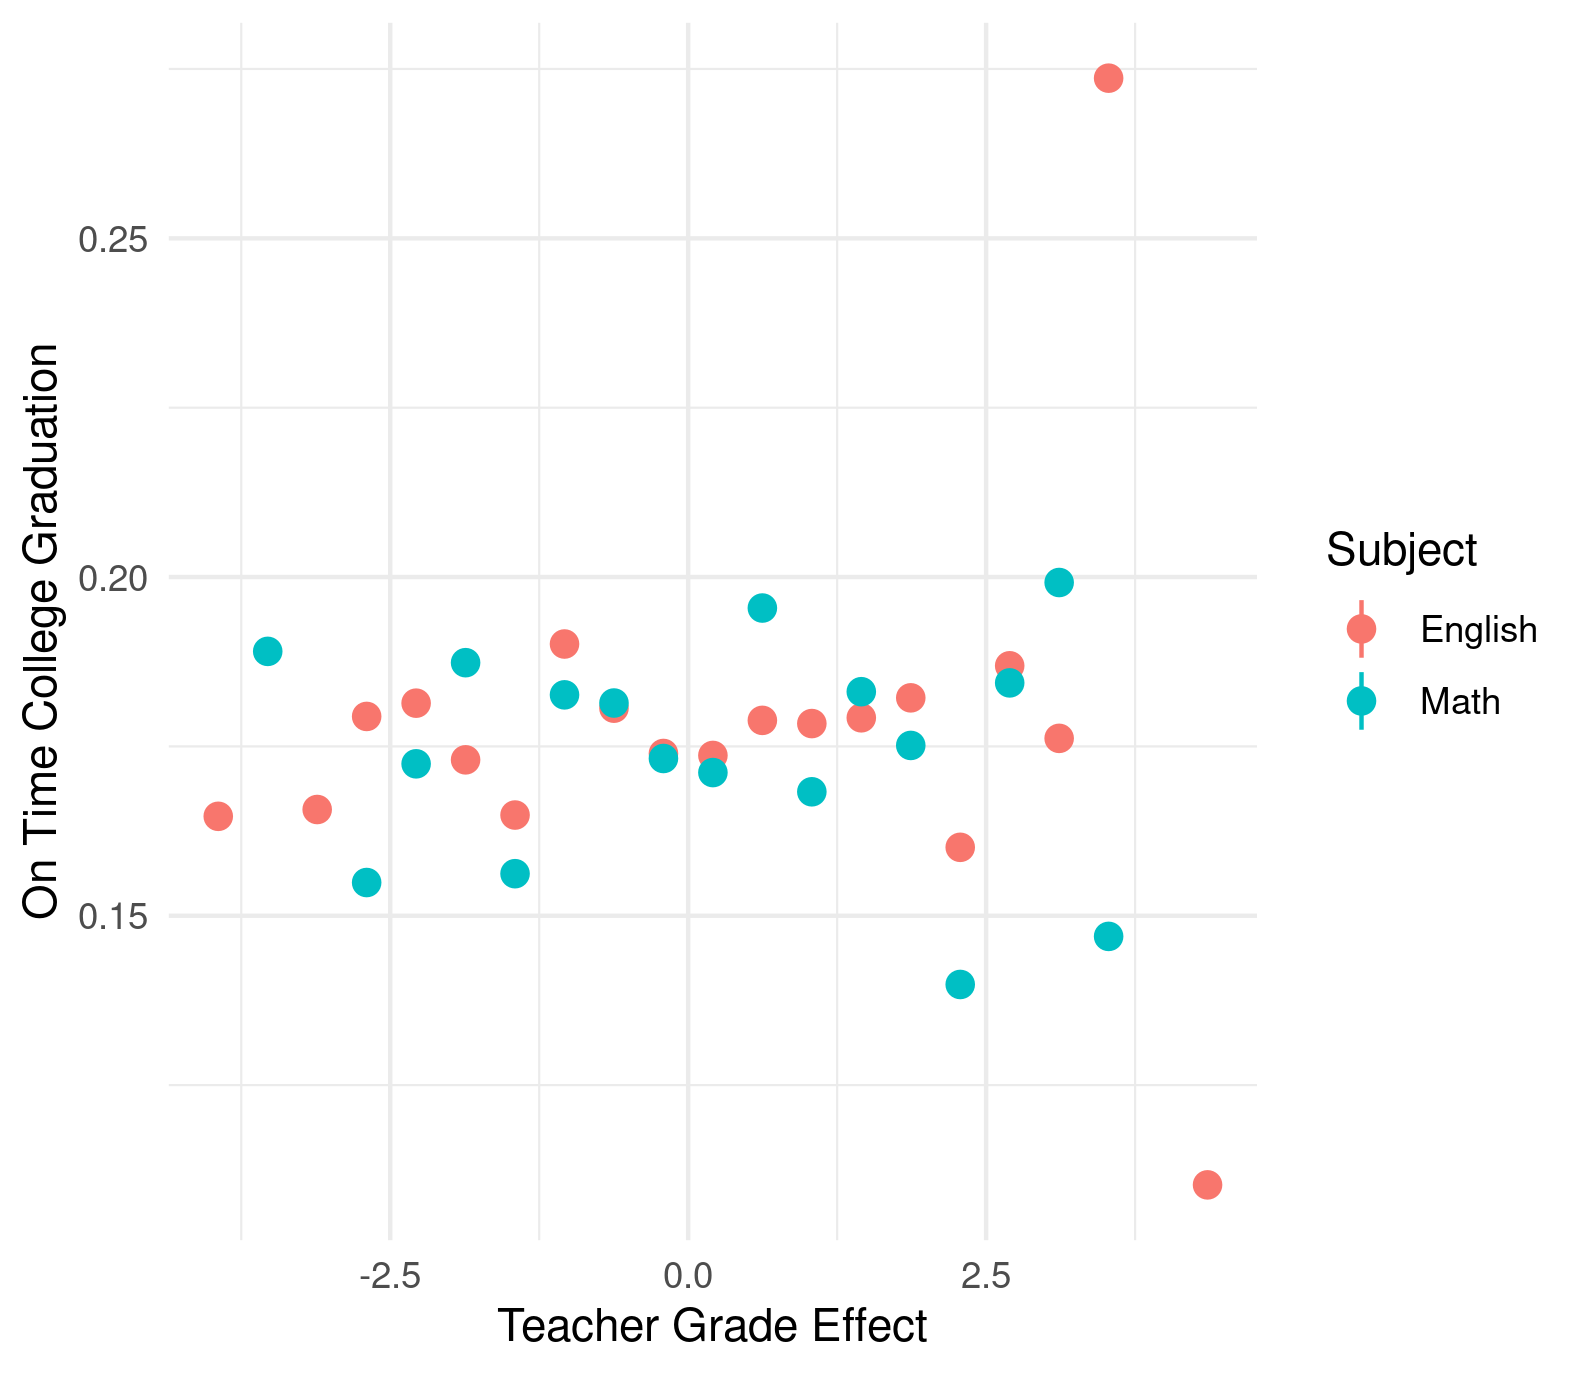
\includegraphics[width=\textwidth]{/Users/roymckenzie/Dropbox/Thesis/ECON/Output/on_time_graduation_scatter.png}
         \caption{On Time College Graduation}
         \label{fig:on_time_graduation}
     \end{subfigure}
    \caption{Post-Secondary Outcomes}
    \label{fig:long}
\end{figure}


\end{document}